\subsection{Case Study 2 — Inverted Pendulum on a Cart}

The inverted pendulum on a cart stands as perhaps the most iconic example of an inherently unstable dynamical system in control engineering education and research. This system consists of a pendulum attached to a motorized cart that can move horizontally, with the control objective being to balance the pendulum in its upright equilibrium position despite the constant influence of gravity pulling it toward the stable downward position. While the physics governing this system can be described in a single paragraph, the mathematical derivation reveals the rich coupling between the cart's translational motion and the pendulum's rotational motion, and demonstrates why systematic modeling techniques are essential for control design.

\begin{figure}[htbp]
\centering
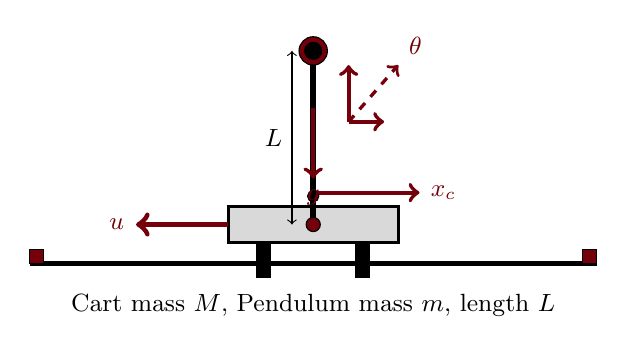
\begin{tikzpicture}[scale=0.9, every node/.style={font=\small}]
    % Define UofSC colors
    \definecolor{UofSCGarnet}{RGB}{115,0,10}
    \definecolor{UofSCBlack}{RGB}{0,0,0}

    % Ground
    \draw[line width=1.5pt, UofSCBlack] (-4, 0) -- (4, 0);
    \draw[fill=UofSCGarnet] (-4, 0) rectangle (-3.8, 0.2);
    \draw[fill=UofSCGarnet] (3.8, 0) rectangle (4, 0.2);

    % Cart
    \draw[fill=gray!30, draw=UofSCBlack, line width=1pt] (-1.2, 0.3) rectangle (1.2, 0.8);
    \draw[fill=UofSCBlack] (-0.8, 0.3) rectangle (-0.6, -0.2);
    \draw[fill=UofSCBlack] (0.6, 0.3) rectangle (0.8, -0.2);

    % Cart coordinate
    \draw[->, UofSCGarnet, line width=1.5pt] (0, 1) -- (1.5, 1) node[right] {$x_c$};
    \draw[fill=UofSCGarnet] (0, 0.95) circle (0.08);

    % Pendulum
    \draw[line width=2pt, UofSCBlack] (0, 0.55) -- (0, 3);
    \draw[fill=UofSCGarnet] (0, 3) circle (0.2);
    \draw[fill=UofSCGarnet] (0, 0.55) circle (0.1);

    % Pendulum angle
    \draw[->, UofSCGarnet, line width=1.5pt] (0.5, 2) -- (1, 2);
    \draw[->, UofSCGarnet, line width=1.5pt] (0.5, 2) -- (0.5, 2.8);
    \draw[->, UofSCGarnet, line width=1.2pt, dashed] (0.5, 2) -- (1.2, 2.8) node[above right] {$\theta$};

    % Mass center
    \draw[fill=UofSCBlack] (0, 3) circle (0.12);

    % Force arrow
    \draw[->, UofSCGarnet, line width=2pt] (-1.2, 0.55) -- (-2.5, 0.55) node[left] {$u$};

    % Length annotation
    \draw[<->, UofSCBlack] (-0.3, 0.55) -- (-0.3, 3) node[midway, left] {$L$};

    % Gravity arrow
    \draw[->, UofSCGarnet, line width=1.5pt] (0, 2.2) -- (0, 1.2) node[below] {$g$};

    % Labels
    \node[below] at (0, -0.3) {Cart mass $M$, Pendulum mass $m$, length $L$};
\end{tikzpicture}
\caption{Inverted pendulum on a cart system with coordinate definitions.}
\label{fig:inverted_pendulum_schematic}
\end{figure}

We begin by precisely defining the system configuration and coordinates. Consider a cart of mass $M$ that slides frictionlessly on a horizontal track. Attached to the cart at point $(x_c, 0)$ is a uniform rod of mass $m$ and length $L$ that pivots freely at the cart. The position of the cart along the track is denoted by $x_c(t)$, and the angle of the pendulum from the vertical upward direction is denoted by $\theta(t)$, where $\theta = 0$ corresponds to the perfectly upright (unstable) equilibrium. The cart is actuated by a horizontal force $u(t)$ applied by a motor, and this force is our control input. The goal of the control system is to determine $u(t)$ as a function of measured quantities such that the pendulum remains balanced near $\theta = 0$ even when subjected to disturbances.

To derive the equations of motion, we employ Lagrangian mechanics, a powerful framework that systematically accounts for energy transformations in mechanical systems. The Lagrangian $ \mathcal{L} $ is defined as the difference between the system's kinetic energy $T$ and potential energy $V$: $\mathcal{L} = T - V$. The equations of motion follow from the Euler-Lagrange equation $\frac{d}{dt}\left(\frac{\partial \mathcal{L}}{\partial \dot{q}_i}\right) - \frac{\partial \mathcal{L}}{\partial q_i} = Q_i$, where $q_i$ represents each generalized coordinate and $Q_i$ represents the generalized force associated with that coordinate.

Our system has two degrees of freedom, so we choose the generalized coordinates $q_1 = x_c$ (the cart position) and $q_2 = \theta$ (the pendulum angle). The first step in the Lagrangian approach is to express the kinetic and potential energies in terms of these coordinates and their time derivatives.

The cart moves purely in the horizontal direction, so its kinetic energy is simply $T_{\text{cart}} = \frac{1}{2}M\dot{x}_c^2$. The pendulum, however, has both translational and rotational kinetic energy. The center of mass of the pendulum is located at a distance $L/2$ from the pivot point. The coordinates of the pendulum's center of mass are given by the horizontal position $x_c + \frac{L}{2}\sin\theta$ and the vertical position $\frac{L}{2}\cos\theta$. Differentiating with respect to time, the velocity components of the pendulum center of mass are $\dot{x}_{\text{pend}} = \dot{x}_c + \frac{L}{2}\dot{\theta}\cos\theta$ in the horizontal direction and $\dot{y}_{\text{pend}} = -\frac{L}{2}\dot{\theta}\sin\theta$ in the vertical direction.

The translational kinetic energy of the pendulum is therefore $T_{\text{trans}} = \frac{1}{2}m\left(\dot{x}_{\text{pend}}^2 + \dot{y}_{\text{pend}}^2\right)$. Substituting the velocity expressions and simplifying, we obtain:
\begin{equation}
T_{\text{trans}} = \frac{1}{2}m\left[\left(\dot{x}_c + \frac{L}{2}\dot{\theta}\cos\theta\right)^2 + \left(-\frac{L}{2}\dot{\theta}\sin\theta\right)^2\right].
\end{equation}

Expanding this expression and collecting like terms:
\begin{equation}
T_{\text{trans}} = \frac{1}{2}m\left[\dot{x}_c^2 + L\dot{x}_c\dot{\theta}\cos\theta + \frac{L^2}{4}\dot{\theta}^2\cos^2\theta + \frac{L^2}{4}\dot{\theta}^2\sin^2\theta\right] = \frac{1}{2}m\left[\dot{x}_c^2 + L\dot{x}_c\dot{\theta}\cos\theta + \frac{L^2}{4}\dot{\theta}^2\right].
\end{equation}

The rotational kinetic energy of the pendulum about its center of mass is $T_{\text{rot}} = \frac{1}{2}I_{\text{cm}}\dot{\theta}^2$, where $I_{\text{cm}} = \frac{1}{12}mL^2$ is the moment of inertia of a uniform rod about its center. Thus $T_{\text{rot}} = \frac{1}{24}mL^2\dot{\theta}^2$.

Combining the translational and rotational contributions, the total kinetic energy of the pendulum is:
\begin{equation}
T_{\text{pend}} = \frac{1}{2}m\dot{x}_c^2 + \frac{1}{2}mL\dot{x}_c\dot{\theta}\cos\theta + \frac{1}{2}m\frac{L^2}{4}\dot{\theta}^2 + \frac{1}{24}mL^2\dot{\theta}^2 = \frac{1}{2}m\dot{x}_c^2 + \frac{1}{2}mL\dot{x}_c\dot{\theta}\cos\theta + \frac{7}{48}mL^2\dot{\theta}^2.
\end{equation}

The total kinetic energy of the entire system is the sum of the cart and pendulum kinetic energies:
\begin{equation}
T = T_{\text{cart}} + T_{\text{pend}} = \frac{1}{2}M\dot{x}_c^2 + \frac{1}{2}m\dot{x}_c^2 + \frac{1}{2}mL\dot{x}_c\dot{\theta}\cos\theta + \frac{7}{48}mL^2\dot{\theta}^2.
\end{equation}

Grouping terms, we write this in the compact form:
\begin{equation}
T = \frac{1}{2}(M + m)\dot{x}_c^2 + \frac{1}{2}mL\dot{x}_c\dot{\theta}\cos\theta + \frac{7}{48}mL^2\dot{\theta}^2.
\end{equation}

The potential energy of the system depends only on the vertical position of the pendulum's center of mass. Setting the zero of potential energy at the track level ($y = 0$), the potential energy is $V = mgy_{\text{pend}} = mg\left(\frac{L}{2}\cos\theta\right) = \frac{1}{2}mgL\cos\theta$. The cart has no potential energy since it moves horizontally at constant height.

We now have all the components needed to construct the Lagrangian:
\begin{equation}
\mathcal{L} = T - V = \frac{1}{2}(M + m)\dot{x}_c^2 + \frac{1}{2}mL\dot{x}_c\dot{\theta}\cos\theta + \frac{7}{48}mL^2\dot{\theta}^2 - \frac{1}{2}mgL\cos\theta.
\end{equation}

To derive the equations of motion, we apply the Euler-Lagrange equation for each generalized coordinate. We begin with the cart coordinate $x_c$. The partial derivatives are:
\begin{equation}
\frac{\partial \mathcal{L}}{\partial \dot{x}_c} = (M + m)\dot{x}_c + \frac{1}{2}mL\dot{\theta}\cos\theta,
\end{equation}
\begin{equation}
\frac{d}{dt}\left(\frac{\partial \mathcal{L}}{\partial \dot{x}_c}\right) = (M + m)\ddot{x}_c + \frac{1}{2}mL\ddot{\theta}\cos\theta - \frac{1}{2}mL\dot{\theta}^2\sin\theta,
\end{equation}
\begin{equation}
\frac{\partial \mathcal{L}}{\partial x_c} = 0.
\end{equation}

The generalized force associated with $x_c$ is the applied control force $u$, so $Q_{x_c} = u$. The Euler-Lagrange equation for $x_c$ is therefore:
\begin{equation}
(M + m)\ddot{x}_c + \frac{1}{2}mL\ddot{\theta}\cos\theta - \frac{1}{2}mL\dot{\theta}^2\sin\theta = u.
\end{equation}

This equation relates the cart acceleration to the pendulum dynamics through the coupling term involving $\ddot{\theta}$ and the centrifugal term involving $\dot{\theta}^2$. We will simplify this equation shortly after deriving the second equation.

For the pendulum coordinate $\theta$, the partial derivatives are:
\begin{equation}
\frac{\partial \mathcal{L}}{\partial \dot{\theta}} = \frac{1}{2}mL\dot{x}_c\cos\theta + \frac{7}{24}mL^2\dot{\theta},
\end{equation}
\begin{equation}
\frac{d}{dt}\left(\frac{\partial \mathcal{L}}{\partial \dot{\theta}}\right) = \frac{1}{2}mL\ddot{x}_c\cos\theta - \frac{1}{2}mL\dot{x}_c\dot{\theta}\sin\theta + \frac{7}{24}mL^2\ddot{\theta},
\end{equation}
\begin{equation}
\frac{\partial \mathcal{L}}{\partial \theta} = -\frac{1}{2}mL\dot{x}_c\dot{\theta}\sin\theta + \frac{1}{2}mgL\sin\theta.
\end{equation}

There are no explicit generalized forces applied to the pendulum angle (it is free to rotate on its pivot), so $Q_\theta = 0$. The Euler-Lagrange equation for $\theta$ gives:
\begin{equation}
\frac{1}{2}mL\ddot{x}_c\cos\theta - \frac{1}{2}mL\dot{x}_c\dot{\theta}\sin\theta + \frac{7}{24}mL^2\ddot{\theta} + \frac{1}{2}mL\dot{x}_c\dot{\theta}\sin\theta - \frac{1}{2}mgL\sin\theta = 0.
\end{equation}

Notice that the terms $-\frac{1}{2}mL\dot{x}_c\dot{\theta}\sin\theta$ and $+\frac{1}{2}mL\dot{x}_c\dot{\theta}\sin\theta$ cancel each other, simplifying the equation considerably:
\begin{equation}
\frac{1}{2}mL\ddot{x}_c\cos\theta + \frac{7}{24}mL^2\ddot{\theta} - \frac{1}{2}mgL\sin\theta = 0.
\end{equation}

We can multiply this entire equation by $2/(mL)$ to simplify the coefficients:
\begin{equation}
\ddot{x}_c\cos\theta + \frac{7}{12}L\ddot{\theta} - g\sin\theta = 0.
\end{equation}

We now have a system of two coupled second-order nonlinear differential equations:
\begin{equation}
(M + m)\ddot{x}_c + \frac{1}{2}mL\ddot{\theta}\cos\theta - \frac{1}{2}mL\dot{\theta}^2\sin\theta = u,
\end{equation}
\begin{equation}
\ddot{x}_c\cos\theta + \frac{7}{12}L\ddot{\theta} - g\sin\theta = 0.
\end{equation}

These equations fully describe the dynamics of the inverted pendulum on a cart. However, for control design purposes, we typically linearize these equations about the operating point of interest. For the inverted pendulum, the operating point is the unstable equilibrium at $\theta = 0$ (upright), $\dot{\theta} = 0$ (no rotation), and $\dot{x}_c = 0$ (cart stationary). At this operating point, $\sin\theta \approx \theta$, $\cos\theta \approx 1$, and terms involving $\dot{\theta}^2$ are second-order small quantities that we neglect.

Applying these approximations to the nonlinear equations, we obtain the linearized equations of motion:
\begin{equation}
(M + m)\ddot{x}_c + \frac{1}{2}mL\ddot{\theta} = u,
\end{equation}
\begin{equation}
\ddot{x}_c + \frac{7}{12}L\ddot{\theta} - g\theta = 0.
\end{equation}

These linear equations capture the essential dynamics of the inverted pendulum near the upright equilibrium and are much more amenable to analysis and control design than the original nonlinear equations.

To develop a state-space model, we first solve the linearized equations for the accelerations $\ddot{x}_c$ and $\ddot{\theta}$ in terms of the states and input. From the second equation, we have $\ddot{x}_c = - \frac{7}{12}L\ddot{\theta} + g\theta$. Substituting this into the first equation:
\begin{equation}
(M + m)\left(- \frac{7}{12}L\ddot{\theta} + g\theta\right) + \frac{1}{2}mL\ddot{\theta} = u.
\end{equation}

Expanding and collecting terms with $\ddot{\theta}$:
\begin{equation}
-\frac{7}{12}(M + m)L\ddot{\theta} + (M + m)g\theta + \frac{1}{2}mL\ddot{\theta} = u,
\end{equation}
\begin{equation}
\left[-\frac{7}{12}(M + m) + \frac{1}{2}m\right]L\ddot{\theta} + (M + m)g\theta = u.
\end{equation}

The coefficient of $\ddot{\theta}$ simplifies as follows:
\begin{equation}
-\frac{7}{12}(M + m) + \frac{1}{2}m = -\frac{7}{12}M - \frac{7}{12}m + \frac{6}{12}m = -\frac{7}{12}M - \frac{1}{12}m = -\frac{7M + m}{12}.
\end{equation}

Thus:
\begin{equation}
-\frac{7M + m}{12}L\ddot{\theta} + (M + m)g\theta = u.
\end{equation}

Solving for $\ddot{\theta}$:
\begin{equation}
\ddot{\theta} = \frac{12}{L(7M + m)}\left[(M + m)g\theta - u\right].
\end{equation}

We can also solve for $\ddot{x}_c$ by substituting this expression back into $\ddot{x}_c = - \frac{7}{12}L\ddot{\theta} + g\theta$:
\begin{equation}
\ddot{x}_c = - \frac{7}{12}L \cdot \frac{12}{L(7M + m)}\left[(M + m)g\theta - u\right] + g\theta = - \frac{7}{7M + m}\left[(M + m)g\theta - u\right] + g\theta.
\end{equation}

Simplifying:
\begin{equation}
\ddot{x}_c = -\frac{7(M + m)g\theta}{7M + m} + \frac{7u}{7M + m} + g\theta = \left[-\frac{7(M + m)}{7M + m} + 1\right]g\theta + \frac{7u}{7M + m}.
\end{equation}

The coefficient of $\theta$ simplifies as follows:
\begin{equation}
-\frac{7(M + m)}{7M + m} + 1 = -\frac{7M + 7m}{7M + m} + \frac{7M + m}{7M + m} = \frac{-7M - 7m + 7M + m}{7M + m} = \frac{-6m}{7M + m}.
\end{equation}

Therefore:
\begin{equation}
\ddot{x}_c = -\frac{6m}{7M + m}g\theta + \frac{7}{7M + m}u.
\end{equation}

Now we define the state vector for our system. Since we have two second-order equations, we need four state variables. A natural choice is:
\begin{equation}
\mathbf{x} = \begin{bmatrix} x_1 & x_2 & x_3 & x_4 \end{bmatrix}^T = \begin{bmatrix} x_c & \dot{x}_c & \theta & \dot{\theta} \end{bmatrix}^T.
\end{equation}

The state derivatives are:
\begin{equation}
\dot{x}_1 = \dot{x}_c = x_2,
\end{equation}
\begin{equation}
\dot{x}_2 = \ddot{x}_c = -\frac{6m}{7M + m}g x_3 + \frac{7}{7M + m}u,
\end{equation}
\begin{equation}
\dot{x}_3 = \dot{\theta} = x_4,
\end{equation}
\begin{equation}
\dot{x}_4 = \ddot{\theta} = \frac{12(M + m)g}{L(7M + m)} x_3 - \frac{12}{L(7M + m)}u.
\end{equation}

In standard state-space form $\dot{\mathbf{x}} = A\mathbf{x} + Bu$, the matrices are:
\begin{equation}
A = \begin{bmatrix}
0 & 1 & 0 & 0 \\
0 & 0 & -\frac{6mg}{7M + m} & 0 \\
0 & 0 & 0 & 1 \\
0 & 0 & \frac{12(M + m)g}{L(7M + m)} & 0
\end{bmatrix}, \quad
B = \begin{bmatrix} 0 \\ \frac{7}{7M + m} \\ 0 \\ -\frac{12}{L(7M + m)} \end{bmatrix}.
\end{equation}

If we choose the pendulum angle $\theta$ as the output (a common choice for balancing control), the output equation is $y = C\mathbf{x} + Du$ with:
\begin{equation}
C = \begin{bmatrix} 0 & 0 & 1 & 0 \end{bmatrix}, \quad D = \begin{bmatrix} 0 \end{bmatrix}.
\end{equation}

This state-space model reveals several important features of the inverted pendulum dynamics. First, notice that the matrix $A$ has a block structure that reflects the coupling between cart and pendulum dynamics. The bottom-right $2 \times 2$ block (rows and columns 3-4) captures the intrinsic dynamics of the pendulum, which we can analyze by considering the case where the cart is fixed ($\ddot{x}_c = 0$ and $\dot{x}_c = 0$). Setting $x_2 = 0$ and $u = 0$ in the state equations, the pendulum dynamics simplify to:
\begin{equation}
\begin{bmatrix} \dot{x}_3 \\ \dot{x}_4 \end{bmatrix} = \begin{bmatrix} 0 & 1 \\ \frac{12(M + m)g}{L(7M + m)} & 0 \end{bmatrix} \begin{bmatrix} x_3 \\ x_4 \end{bmatrix}.
\end{equation}

The eigenvalues of this $2 \times 2$ matrix are found from the characteristic equation:
\begin{equation}
\det\begin{bmatrix} -\lambda & 1 \\ \frac{12(M + m)g}{L(7M + m)} & -\lambda \end{bmatrix} = \lambda^2 - \frac{12(M + m)g}{L(7M + m)} = 0.
\end{equation}

Thus $\lambda = \pm \sqrt{\frac{12(M + m)g}{L(7M + m)}}$. For a typical inverted pendulum with $M \gg m$, this simplifies to $\lambda \approx \pm \sqrt{\frac{12g}{7L}}$. The positive eigenvalue indicates that the upright equilibrium is exponentially unstable, meaning any small deviation from vertical will grow exponentially over time. This is the fundamental challenge of the inverted pendulum: without control action, the system naturally diverges from the desired operating point.

The full $4 \times 4$ system matrix has eigenvalues that can be determined by solving the characteristic equation $\det(sI - A) = 0$. Computing this determinant:
\begin{equation}
\det\begin{bmatrix}
s & -1 & 0 & 0 \\
0 & s & \frac{6mg}{7M + m} & 0 \\
0 & 0 & s & -1 \\
0 & 0 & -\frac{12(M + m)g}{L(7M + m)} & s
\end{bmatrix} = s^2 \left[s^2 - \frac{12(M + m)g}{L(7M + m)}\right] - \frac{6mg}{7M + m} \cdot \frac{12(M + m)g}{L(7M + m)} s.
\end{equation}

After simplification, the characteristic equation is:
\begin{equation}
s\left[s^3 - \frac{12(M + m)g}{L(7M + m)}s - \frac{72mg}{L(7M + m)^2}\right] = 0.
\end{equation}

One eigenvalue is always at $s = 0$, corresponding to the cart position $x_c$ being an unobservable mode (we can add or subtract a constant from $x_c$ without affecting the dynamics). The remaining cubic equation has two unstable roots (positive real parts) and one stable root (negative real part). The presence of unstable poles means the open-loop system is not stabilizable by simply letting go—the pendulum will fall, and the cart will respond to the coupling in ways that cannot counteract the instability.

The control design problem for the inverted pendulum is now clear: we must design a feedback controller that shifts all poles of the system to the left half-plane (negative real parts), thereby stabilizing the inherently unstable equilibrium. This is achievable through state feedback, where we measure all four states (or estimate them from available measurements) and compute the control input as a linear combination:
\begin{equation}
u = -K_1 x_c - K_2 \dot{x}_c - K_3 \theta - K_4 \dot{\theta}.
\end{equation}

The gains $K_1, K_2, K_3, K_4$ are chosen such that the closed-loop system matrix $A - BK$ has all eigenvalues with negative real parts. This is the pole placement problem we will address in detail in later chapters.

\begin{example}{Linearized Inverted Pendulum Dynamics — Numerical Illustration}
Consider an inverted pendulum with the following physical parameters: cart mass $M = 1$ kg, pendulum mass $m = 0.2$ kg, pendulum length $L = 0.5$ m, and gravitational acceleration $g = 9.81$ m/s². Substituting these values into our linearized model, we first compute the coefficients.

The denominator appearing throughout our equations is $7M + m = 7(1) + 0.2 = 7.2$ kg. The state-space matrices become:
\begin{equation}
A = \begin{bmatrix}
0 & 1 & 0 & 0 \\
0 & 0 & -9.81 & 0 \\
0 & 0 & 0 & 1 \\
0 & 0 & 49.05 & 0
\end{bmatrix}, \quad
B = \begin{bmatrix} 0 \\ 0.9722 \\ 0 \\ -3.333 \end{bmatrix}.
\end{equation}

Computing the eigenvalues of the open-loop $A$ matrix, we find $\lambda = 0$, $\lambda = -7.00$, and $\lambda = \pm 7.00$. The pair of purely imaginary eigenvalues at $\pm 7.00$ (in this simplified case where $M \gg m$) indicates marginal instability—if the pendulum tips, it will oscillate with increasing amplitude. The zero eigenvalue corresponds to the fact that the absolute cart position doesn't affect the dynamics; only relative motion matters.

If we design a state feedback controller with gains $K = \begin{bmatrix} -1.5 & -4.0 & -60.0 & -10.0 \end{bmatrix}$, the closed-loop system has eigenvalues at approximately $\lambda = -2.0$, $\lambda = -3.0$, and $\lambda = -5.0 \pm 2.5j$. All eigenvalues have negative real parts, confirming that the closed-loop system is stable. The gains can be interpreted physically: $K_3 = -60$ provides strong feedback proportional to the pendulum angle (correct more aggressively for larger deviations from vertical), $K_4 = -10$ provides damping proportional to angular velocity (resist rapid swinging motion), and the cart-related gains help maintain the cart near some reference position while managing the coupling between the two degrees of freedom.
\end{example}

The inverted pendulum illustrates several fundamental principles that recur throughout control systems engineering. First, accurate mathematical modeling is not optional—it is essential. The coupling between cart and pendulum dynamics means that a controller designed for a simplified model (ignoring the cart dynamics, for instance) will fail dramatically when applied to the actual system. Second, unstable systems require feedback for stabilization; no amount of open-loop planning can maintain an unstable equilibrium in the presence of disturbances. Third, the pole placement approach (choosing desired closed-loop dynamics and computing the required feedback gains) provides a systematic framework for control design, rather than relying on trial and error.

The inverted pendulum also serves as a benchmark problem for testing control algorithms. Its apparent simplicity (just two degrees of freedom, one input) belies the depth of analysis required to understand and control it. Variations of this problem—inverted pendulum on a moving cart, double inverted pendulum, inverted pendulum with time delays or nonlinear friction—continue to be active areas of research and serve as stepping stones to more complex real-world control challenges such as rocket launch vehicle stabilization, humanoid robot balance, and spacecraft attitude control.
